\chapter{New method for Bayesian computation: using sequential Monte Carlo and
  Path sampling}
\label{cha:New method for Bayesian computation}

As already introduced through chapter~\ref{cha:Bayesian model selection}, the
main interest is to estimate the Bayesian factor. In more general setting, it
is the same as estimating the ratio of normalizing constants. In this chapter,
we propose a new method for the estimation, namely using sequential Monte
Carlo techniques and path sampling identity.

The sequential Monte Carlo (\smc) technique constructs an importance
distribution for a target distribution of interest iteratively. The basic idea
is that starting from a distribution which is easy to sample from or
approximated by an importance distribution, and iteratively, move the
importance distribution towards the target distribution of interest. The
distributions constructed by the intermediate steps can be used to estimate
the ratio of normalizing constants between the target and initial
distribution. \parencite{DelMoral2006}

The path sampling technique constructs a continuous \emph{path} to bridge two
distributions, and estimates the logarithm ratio of normalizing constants
between the distributions by an simple identity introduced in
section~\ref{sec:Path sampling estimator}. The exact meaning of ``path'' will
be introduced in the same section. However, it is worth mention here that,
when implementing the path sampling estimator, this path is often constructed
as a sequence of distributions and numerical integration is used to
approximate the estimator. See section~\ref{sec:Path sampling estimator}.
\parencite{Gelman1998}

These two techniques can be combined together for the estimating of ratios of
normalizing constants. One way to think of it is that, the path sampling
estimator is one of the ways to use the output from a \smc algorithm to
estimate the (logarithm) ratio of normalizing constants. The other way to
think of it is that, the \smc algorithm provides a simple way to construct a
sequence of distributions, which can be used to approximate the expectations
with respect to each of the distribution in a given sequence (the ``path'' of
path sampling) through importance sampling.

In section~\ref{sec:smc algorithm}, the \smc algorithm is introduced. In the
following section~\ref{sec:Path sampling estimator}, the path sampling
identity is presented. What follows is a simple example is provided to
illustrate the idea. This chapter is completed by a discussion of future
research direction for the proposed method.

\section{\smc algorithm}
\label{sec:smc algorithm}

In this section, the \smc algorithm is introduced. Consider a sequence of
distributions indexed by discrete time $n$, say $\pi_n$. Usually the
distributions are known up to a normalizing constant, say $Z_n$, and $\pi_n
= \gamma_n/Z_n$. The \smc algorithm is based on the sequential importance
sampling techniques. At time $n = 1$, we start with $\pi_1$ and construct an
efficient importance distribution, say $\eta_1$, and we sample $N$ random
numbers from distribution $\eta_1$, called particles. At time $n > 1$,
suppose we have $N$ particles following distribution $\eta_{n-1}$, and we
move these particles in a sensible way to a new distribution $\eta_n$ such
that $\eta_n$ is an efficient importance distribution for $\pi_n$. This is
done by moving the $N$ particles by a sensible Markov kernel $K_n$ such that
particles are moved into high density region of $\pi_n$. This technique is
called sequential importance sampling in some literature
\parencite[e.g.][]{DelMoral2006}.

It should be intuitively clear that, in general to do any kind of estimations,
we need be able to evaluate the importance weights at each time $n$, and thus
$\eta_n$ need to be evaluated point-wise. Typically this is impossible in many
situations. Note that
\begin{equation}
  \eta_n(x_n) = \int\eta_1(x_1)\prod_{j=2}^nK_j(x_{j-1},x_j) \dd x_{1:n-1}.
  \label{eq:marginal importance}
\end{equation}
And if the kernel $K_j$ in the integration is constructed by an \mha, it can
be difficult to compute $K_j$ point-wise, and thus the integral. The \smc
algorithm introduce an auxiliary backward Markov chain kernel to solve this
problem for the case where all $E_n$ has the same dimension. The purpose of
the backward kernel is that by construction, the target distributions increase
in dimension while they admit $\pi_n$'s as their marginal distributions.

In the presentations below, it will be made clear that, the computation of
importance weights is made possible by introducing this auxiliary backward
kernel. At each time $n$, let $L_{n-1}(x_n,x_{n-1})$ be a Markov kernel. It
is called backward in the sense that it is a transition kernel from $x_n$ to
$x_{n-1}$, which is backward in time. And construct,
\begin{equation}
  \tilde{\pi}_n(x_{1:n}) = \frac{\tilde{\gamma}_n(x_{1:n})}{Z_n}
\end{equation}
where $x_{1:n} = (x_1,\dots,x_n)^T$, $Z_n$ is the normalizing constants of
both $\gamma_n$ and $\tilde{\gamma}_n$, and
\begin{equation}
  \tilde{\gamma}_n(x_{1:n}) = \gamma_n(x_n)
  \prod_{k=1}^{n-1}L_k(x_{k+1},x_k).
\end{equation}
By construction, the new target distribution $\tilde{\pi}_n$ satisfies the
requirement for standard sequential importance sampling, and admit $\pi_n$
as its marginal distribution. Therefore any estimates about $\pi_n$ can be
done through sampling from $\tilde{\pi}_n$.

Now back to the standard sequential importance sampling scheme, at time
$n=1$, we have $\eta_1$ as an importance distribution for $\tilde{\pi}_1 =
\pi_1$. Also $N$ particles are sampled, say, $\{X_1^{(i)}\}$. And a set of
corresponding weights $\{W_1^{(i)}\}$ are calculated by,
\begin{align}
  w_1^{(i)} =
  w_1(X_1^{(i)}) &= \frac{\gamma_1(X_1^{(i)})}{\eta_1(X_1^{(i)})}
  \label{eq:ini_weight}\\
  W_1^{(i)} =
  W_1(X_1^{(i)}) &= \frac{w_1(X_1^{(i)})}{\sum_{j=1}^Nw_1(X_1^{(j)})}
  \label{eq:ini_weight_norm}
\end{align}
At time $n-1$, we have a set of weights and particles, $\{W_{n-1}^{(i)},
  X_{n-1}^{(i)}\}$, and move the particles by Markov kernel $K_n(x_{n-1},
x_n)$. Then the new weight for particle $x_{1:n}$ will be,
\begin{align}
  w_n(x_{1:n}) &= \frac{\tilde{\gamma}_n(x_{1:n})}{\eta_n(x_{1:n})}
  \allowdisplaybreaks\notag\\
  &= \frac{\gamma_n(x_n)\prod_{k=1}^{n-1}L_k(x_{k+1},x_k)}
  {\eta_{n-1}(x_{1:n-1})K_n(x_{n-1},x_n)}
  \frac{\gamma_{n-1}(x_{n-1})}{\gamma_{n-1}(x_{n-1})} \notag\\
  &= \frac{\gamma_n(x_n)L_{n-1}(x_n,x_{n-1})\tilde{\gamma}_{n-1}(x_{n-1})}
  {\gamma_{n-1}(x_{n-1})\eta_{n-1}(x_{1:n-1})K_n(x_{n-1},x_n)} \notag\\
  &= w_{n-1}(x_{1:n-1})\tilde{w}_n(x_{n-1},x_n),
\end{align}
where,
\begin{equation}
  \tilde{w}_n(x_{n-1},x_n) =
  \frac{\gamma_n(x_n)L_{n-1}(x_n,x_{n-1})}
  {\gamma_{n-1}(x_{n-1})K_n(x_{n-1},x_n)}.
  \label{eq:incr_weight}
\end{equation}
Applying the above equation for particles $\{W_{n-1}^{(i)}, X_{n-1}^{(i)}\}$
and newly generated $\{X_n^{(i)}\}$, the incremental weights ($\tilde{w}$)
and normalized weights $\{W_n^{(i)}\}$ can therefore be calculated.

\paragraph{Degeneracy} The degeneracy problem mentioned earlier can be
measured by the variance of the normalized weights, as similar in the case
of regular importance sampling. Intuitively, as the time index $n$
increases, the discrepancy between $\eta_n$ and $\tilde{\pi}_n$ increases as
well, and the variance of the normalized important weights tends to
increase.

One way to solve this problem is to resample the particles. The resampling
process consists of selecting new particles and weights such that the
discrepancy is reduced. The resampled particles should also be as good an
approximation to the distribution $\pi_n$ as possible \parencite{Douc2005}.
There are a number of resampling schemes. One class of them is under the
constrains that, each particle $\{X_n^{(i)}\}$ is copied $N_n^{(i)}$ times,
such that $\sum_{i=1}^N N_n^{(i)} = N$, $\Exp[N_n^{(i)}|X_{1:n}] =
NW_n^{(i)}$ and the new particle set has equal weights
\parencite{Douc2005,DelMoral2006}.

To decide when to perform resampling, one can define \ess as
$(\sum_{i=1}^N(W_n^{(i)})^2)^{-1}$, and it can be used as a criterion for
whether or not resampling is required at time $n$ \parencite{Liu1998}.
Intuitively, with the discrepancy between $\eta_n$ and $\pi_n$ increasing,
many particulars will have smaller and smaller weights. Carrying on a lot of
particulars with very small weights is apparently a waste. In this sense, it
is sensible to use a quality measuring the variance of normalized weights to
decide when to do resampling, since the mean of normalized weights is fixed to
be $1/N$. Mathematically, it was argued in \textcite{Liu1998} that the
effective sample size (\ess) is approximately proportional to the inverse of
the variance of importance sampling estimator associated with the weights. And
therefore it is used as an indicator of requirement of resampling.

\paragraph{Summary of the algorithm} In short the algorithm for a sequence
$\pi_n$, $n = 1,\dots,p$, can be represented as below,
\parencite{DelMoral2006}
\begin{enumerate}
  \item Set $n=1$, draw $X_1^{(i)}$ from $\eta_1$ for $i = 1,\dots,N$.  And
    evaluate $\{W_1^{(i)}\}$ by equations~\eqref{eq:ini_weight}
    and~\eqref{eq:ini_weight_norm}.
  \item If $\ESS < T$, where $T$ is a predefined threshold, resample.
  \item Set $n = n + 1$, if $n = p + 1$, stop and exit the algorithm.
    Otherwise, draw $X_n^{(i)}$ from $K_n(X_{n-1}^{(i)},\cdot)$, and compute
    $\{\tilde{w}_n(X_{n-1}^{(i)},
      X_n^{(i)}\}$ by equation~\eqref{eq:incr_weight}. The new normalized
    weights, $\{W_n^{(i)}\}$ is computed by
    \begin{equation}
      W_n^{(i)} = \frac{W_{n-1}^{(i)}\tilde{w}_n(X_{n-1}^{(i)},X_n^{(i)})}
      {\sum_{j=1}^NW_{n-1}^{(j)}\tilde{w}_n(X_{n-1}^{(j)},X_n^{(j)})}
    \end{equation}
  \item Go to step 3.
\end{enumerate}

A few problems remains here to actually implement the algorithm. First is
the choice of the kernel $K_n$.  The second problem is the optimization of
the backward kernel $L_{n-1}$.

\subsection{Choice of forward kernels}
\label{sub:Choice of forward kernels}

In general, if resampling is not performed at each iteration, then between two
resampling steps, the \smc algorithm construct $N$ inhomogeneous Markov chains
$\{X_{1:n}^{(i)}\}$. In most cases the marginal distributions for $X_{1:n}$,
$\eta_n \ne \pi_n$. As similar to regular importance sampling, the optimal
forward kernel (also called proposal) is that $K_n(x_{n-1},x_n) = \pi_n(x_n)$
in the sense of minimizing variance of the estimator. This choice is clearly
impossible (or otherwise the \smc method is entirely unneeded). A few classes
of kernels was used in the literature.

\paragraph{Independent proposals} It is possible to construct
$K_n(x_{n-1},x_n) = K_n(x_n)$ where $K_n$ is a density function. The
parameters can be determined by using information from $\{X_{n-1}^{(i)}\}$
\parencite[e.g.][]{West1993}. Independent proposals appear to be dependent on
good behavior of the sequence $\{\pi_n\}$. One way to construct proposals
adaptively is proposed by \textcite{Jasra2008}. However, it is still difficult
to construct independent proposals which approximate $\pi_n$ well in many
cases. For example, with a multi modes $\pi_n$, a standard distribution like
Normal can hardly be efficient. Therefore, it is sensible to construct local
moves.

\paragraph{Local random-walk moves} An alternative to above is using
$K_n(x_{n-1},x_n)$ a random-walk kernel \parencite[e.g.][]{Givens1996}.  It
worth noting that the local random-walk here is very different from the
Metropolis random-walk. In the \mcmc case, The entire sequence of random-walks
explores a single target distribution and past moves provide information about
this distribution. In contrast, in the \smc case, at each iteration, the
target is a new distribution $\pi_n$ and information about this distribution
is not used in many situations unless $\pi_n$ is close enough to $\pi_{n-1}$.

\paragraph{Markov chain Monte Carlo moves} As proposed in
\textcite{DelMoral2006}, it is natural to set $K_n$ as an \mcmc kernel of
invariant distribution $\pi_n$. It is sensible in the cases either $K_n$
mixes fast enough or $\pi_n$ evolves slowly so that we can expect $\eta_n$
to be close to $\pi_n$.

\subsection{Choice of backward kernels}
\label{sub:Choice of backward kernels}

It should be noted that the choice of backward kernel should be optimized
with respect to the chosen forward kernel. Recall that we introduced this
backward kernel to enable the evaluation of weights by doing importance
sampling on space $\prod_{i=1}^n E_i$ (or $E^n$ for the case of common
support $E$) instead of $E_n$. Intuitively the variance of the importance
weights is increased. So the optimal backward kernel will reduce this ``side
effect''. Indeed, as shown in \textcite{DelMoral2006}, the optimal backward
kernel in the sense of minimizing the asymptotic conditional variance of the
estimator if resampling is carried out every iteration is
\begin{equation}
  L_{n-1}^{\mathrm{opt}}(x_n,x_{n-1})
  = \frac{\eta_{n-1}(x_{n-1})K_n(x_{n-1},x_n)}{\eta_n(x_n)}
\end{equation}
and the important weights weights are
\begin{equation}
  w_n(x_{1:n}) = \frac{\gamma_n(x_n)}{\eta_n(x_n)}
\end{equation}
which is exactly the importance sampling weights in marginal space. However,
as for the same reason we need this backward kernel, the above optimal
kernels cannot be computed point-wise, since itself relies on the marginal
distribution $\eta_n$. Several sub-optimal kernels were shown in
\textcite{DelMoral2006}. The one of most interest to this report is as
below.

It was shown that with the \mcmc kernel and $\pi_n$ be close enough to
$\pi_{n-1}$, a good approximation to optimal backward kernel is given by
\begin{equation}
  L_{n-1}(x_n,x_{n-1})
  = \frac{\pi_n(x_{n-1})K_n(x_{n-1},x_n)}{\pi_n(x_n)}.
\end{equation}
In this case,
\begin{equation}
  \tilde{w}_n(x_{n-1},x_n)
  = \frac{\gamma_n(x_{n-1})}{\gamma_{n-1}(x_{n-1})},
\end{equation}
which is particularly easy to compute in many cases.

\subsection{Estimating ratio of normalizing constants}
\label{sub:Estimating ratio of normalizing constants}

The last remark about the \smc algorithm is using the computed weights to
estimate the ratio of normalizing constants, which is of interest to the
Bayesian model comparison problem. The basic identity is
\begin{equation}
  \frac{Z_n}{Z_{n-1}} =
  \frac{\int\gamma_n(x_n)\dd x_n}{\int\gamma_{n-1}(x_{n-1})\dd x_{n-1}}
\end{equation}
and the importance sampling estimates,
\begin{equation}
  \frac{\hat{Z}_n}{Z_{n-1}} =
  \sum_{i=1}^NW_{n-1}^{(i)}\tilde{w}_n(X_{n-1}^{(i)},X_n^{(i)}).
  \label{eq:z_smc}
\end{equation}
To estimate $Z_n/Z_1$, the product of the above estimates can be used. The
formula can be further simplified in the case where resampling is not
performed at each iteration \parencite{DelMoral2006}.

\section{Path sampling estimator}
\label{sec:Path sampling estimator}

The path sampling estimator for the logarithm ratio of normalizing constants
is based on a simple identity. Given a sequence of distributions say,
$\pi_t(\theta)$ known up to normalizing constants, say $\pi_t(\theta) =
\gamma_t(\theta)/Z_t$, where $t$ is a continuous index taken values on
$[0,1]$. The path sampling estimator of the logarithm of ratio of normalizing
constants is based on,
\begin{equation}
  Z_t = \int_{\Theta}\gamma_t(\theta)\dd \theta
\end{equation}
where $\Theta$ is the support of $\theta$. Provided the regularity condition
which allows the change order of integration and differentiation below,
\begin{align}
  \frac{\diff}{\diff t}\log(Z_t)
  &= \frac{1}{Z_t}\frac{\diff}{\diff t}Z_t \notag\\
  &= \int_{\Theta}\frac{1}{Z_t}
  \frac{\diff}{\diff t}\gamma_t(\theta)\dd\theta.
  \label{eq:path_derive1}
\end{align}
Note that
\begin{equation}
  \frac{\diff}{\diff t}\log\gamma_t(\theta)
  = \frac{1}{\gamma_t(\theta)}\frac{\diff}{\diff t}\gamma_t(\theta)
  \quad\text{and}\quad
  \frac{\gamma_t(\theta)}{Z_t} = \pi_t.
\end{equation}
Provided that $\gamma_t(\theta)>0$, substitute the above equations
to~\eqref{eq:path_derive1},
\begin{align}
  \frac{\diff}{\diff t}\log(Z_t)
  &= \int_{\Theta}\log\gamma_t(\theta)\pi_t(\theta)\dd\theta \notag\\
  &= \Exp_t\Square[Big]{\frac{\diff}{\diff t}\log\gamma_t(\theta)}
\end{align}
where the expectation is taken with respect to $\pi_t(\theta)$ with $t$ fixed.
Thus, the path sampling estimator of $\lambda=\log(Z_1/Z_0)$ can be based on
the following identity
\begin{equation}
  \lambda=
  \int_0^1 \Exp_t\Square[Big]{\frac{\diff}{\diff t}\log \gamma_t(\theta)}.
  \label{eq:z_path}
\end{equation}
Note that the index $t$ does not necessarily take values on $[0,1]$, though
for simplicity and without losing generality, this range is used here.

One way to implement the estimator above is interpreting $t$ as a realization
of a uniform random variable $T$ on $[0,1]$. Then the above integration can be
interpreted as the expectation of $(T,\theta)$ on the joint space
$[0,1]\times\Theta$. To obtain an estimate, one can sample from the joint
space of $(T, \Theta)$ and use the simple Monte Carlo approximation.

An alternative way is to use a sequence $0 = t_0 < t_1 < \dots < t_m = 1$, and
numerical integration with trapezoidal rule. In other words, a sequence of
unnormalized distributions $\gamma_{t_n}$ are constructed. If we let
distribution sequence $\{\pi_n\}$ in the \smc setting as described in the
previous section be $\{\gamma_{t_n}/Z_{t_n}\}$, then we can estimate
$\Exp_{t_n}[\frac{\diff}{\diff t_n}\gamma_{t_n}(\theta)]$ by
\begin{equation}
  \Exp_{t_n}[\frac{\diff}{\diff t_n}\gamma_{t_n}(\theta)]
  \approx \sum_{i=1}^NW_n^{(i)}X_n^{(i)},
\end{equation}
where $\{W_n^{(i)},X_n^{(i)}\}$ is the particle set approximating the
expectation of $\pi_n$ as described in the previous section. Denote the right
hand side of above approximation by $U_n$, then we can approximate the path
sampling estimate by
\begin{equation}
  \hat{\lambda} = \sum_{n = 1}^m \frac{1}{2}(t_{n} - t_{n-1})(U_n + U_{n-1})
\end{equation}

\section{Combining sequential Monte Carlo and path sampling}
\label{sec:Combining sequential Monte Carlo and path sampling}

As shown in the end of the last section, there is a way to combine the two
methods together to estimate the ratio or normalizing constants. There are
several motivations for proposing this methods.

First, as any Monte Carlo methods used in Bayesian statistics and other
fields, exploring the distributions (posteriors in Bayesian statistics) is an
important part of the inference process. Sequential Monte Carlo method
provides a solid framework as an alternative to \mcmc for exploring properties
of complex distributions. Further, it can outperform \mcmc in some situations.
For example, for a distribution with multiple modes separated by low
probability areas, a single chain \mha is likely to be slow to explore the
whole parameter space. The \smc algorithm does not suffer this issue provided
a large enough particle set and smooth enough move between iterations.

Second, the path sampling estimator has some attractive properties compared to
harmonic mean estimator described in section~\ref{sub:Importance sampling and
  harmonic mean based estimators} \parencite[see][]{Gelman1998}. It was argued
by those authors as a natural evolution from importance sampling, and we agree
with them on this. However, if we approach the path sampling by simulating
from the joint space of $(T,\theta)$ using existing methods like \mcmc, then
we suffer the same issues discussed in chapter~\ref{cha:Bayesian computation
  with Monte Carlo methods}.

Instead, we propose to combine these two techniques together to obtain a good
estimator for ratio of normalizing constants. In the next section, an example
is constructed to demonstrate the use of the proposed method.

\section{Example}
\label{sec:Example}

To illustrate the use of \smc sampler and path sampling identity for the
estimating of ratio of normalizing constants, consider two models, with
likelihoods as Normal and Laplace (i.e. double exponential) distribution
respectively. Explicitly, model 1, denote by
$\calM_1$, has a likelihood
$\calN(\mu_1,\lambda_1^{-1})$, i.e.,
\begin{equation}
  f(x|\mu_1,\lambda_1) = \sqrt{\frac{\lambda_1}{2\pi}}
  \exp\Curly[Big]{-\frac{\lambda_1(x-\mu_1)^2}{2}}.
\end{equation}
Model 2, denoted by $\calM_2$, has a likelihood of a Laplace distribution,
denoted in this report by $\calL(\mu_2,\lambda_2^{-1})$, i.e.,
\begin{equation}
  f(x|\mu_2,\lambda_2) = \frac{\lambda_2}{2}
  \exp\Curly{-\lambda_2\Abs{x - \mu_2}}
\end{equation}
The Laplace distribution is parameterized in terms of a ``rate'' parameter,
similar to the case of Exponential distribution.

The true data generating mechanism is a mixture of the two distributions.
Explicitly, the true model is written as,
\begin{equation}
  X_i \sim p\calN(0,1) + (1-p)\calL(0, \sqrt{2}/2),
  \label{eq:data_density}
\end{equation}
where $p\in[0,1]$. By construction, the two components have the same variance.
In this example, we will consider two simple case, $p = 0$ or $1$, namely the
data comes from either a Normal distribution or a Laplace distribution.

\subsection{The Normal model}

A conjugate prior is specified for $\calM_1$, the Normal likelihood model.
That is, assuming the data observed are $\x = (x_1,\dots,x_n)^T$,
\begin{align}
  x_i | \mu,\lambda &\sim \calN(x_i; \mu, \lambda^{-1}) \\
  \mu | \mu_0,\lambda,n_0 &\sim \calN(\mu; \mu_0, (n_0\lambda)^{-1}) \\
  \lambda | \alpha,\beta &\sim \calGa(\lambda; \alpha, \beta)
\end{align}
In other words, the prior is a Normal-Gamma distribution with parameters
$(\mu_0, n_0, \alpha, \beta)$. Explicitly, we write the posterior density
as,
\begin{equation}
  \pi(\mu,\lambda|\x) \propto
  L(\mu,\lambda;\x)\pi(\mu,\lambda),
  \label{eq:normal_posterior}
\end{equation}
where
\begin{align}
  L(\mu,\lambda;\x) &= \Round[Big]{\frac{\lambda}{2\pi}}^{n/2}
  \exp\Curly[Big]{-\frac{\lambda}{2}\sum_{i=1}^n(x_i - \mu)^2}
  \label{eq:likelihood_normal}\\
  \pi(\mu,\lambda) &= \sqrt{\frac{n_0\lambda}{2\pi}}
  \exp\Curly[Big]{-\frac{n_0\lambda}{2}(\mu - \mu_0)^2}
  \frac{\beta^{\alpha}}{\Gamma(\alpha)}
  \lambda^{\alpha - 1}\exp\Curly{-\beta\lambda}
  \label{eq:prior_normal}
\end{align}

\subsubsection{Algorithm setting}

Set $\pi_0(\mu,\lambda) = \pi(\mu,\lambda)$, where $\pi(\mu,\lambda)$ is as
in equation~\ref{eq:prior_normal}. Let
\begin{equation}
  \pi_k(\mu,\lambda) \propto (L(\mu,\lambda;\x))^{p_k}\pi_0(\mu,\lambda)
  \label{eq:normal_targets}
\end{equation}
where $L$ is the likelihood function, as in
equation~\eqref{eq:likelihood_normal}, and $\{p_k\in[0,1]\}$ is a sequence
chosen. The \smc sampler starts with $\pi_0$ and the initial importance
distribution is set to be $\pi_0$ as well.

The forward kernel, at step with target $\pi_k$ is constructed as the
following,
\begin{enumerate}
  \item Updating $\lambda$ through multiplicative Log-Normal random-walk
    proposal.
  \item Updating $\mu$ through additive Normal random-walk proposal.
\end{enumerate}
This kernel is constructed such that the random-walk moves mimic the shape of
the target distributions. More specifically, let $\calLN(m,s^2)$ denote the
Log-Normal distribution with parameters $m$ and $s^2$. At time $k$,
corresponding to step $k$, and target $\pi_k(\mu,\lambda)$,
\begin{enumerate}
  \item Given $\lambda_k$, draw $v$ from $\calLN(0,\sigma_{\lambda}^2)$ and
    propose $\lambda_{k+1}=v\lambda_k$.
  \item Given $\mu_k$, draw $u$ from $\calN(0,\sigma_{\mu}^2)$, and propose
    $\mu_{k+1}=\mu_k+u$.
  \item Compute the acceptance probability by
    \begin{equation}
      \delta = \frac{\gamma_{k+1}(\mu_{k+1},\lambda_{k+1})}
      {\gamma_{k+1}(\mu_k,\lambda_k)}v,
      \label{eq:accept_prob}
    \end{equation}
    where $\gamma_k = \pi_k / Z_k$. Accept proposal $(\mu_{k+1},
    \lambda_{k+1})$ with probability $\delta$ as the new particle or
    otherwise copy $(\mu_k, \lambda_k)$ as the value of the new particle.
\end{enumerate}

\begin{remark}
  This is a standard Metropolis random-walk. The acceptance probability is
  derived as following. As in standard rand-walk \mcmc,
  \begin{equation}
    \delta =
    \frac{\gamma_{k+1}(\mu_{k+1},\lambda_{k+1})}
    {\gamma_{k+1}(\mu_k,\lambda_k)}
    \frac{q(\mu_k,\lambda_k|\mu_{k+1},\lambda_{k+1})}
    {q(\mu_{k+1},\lambda_{k+1}|\mu_k,\lambda_k)}
  \end{equation}
  where $q$ is the proposal density. In this case,
  \begin{align}
    q(\mu_{k+1},\lambda_{k+1}|\mu_k,\lambda_k) &=
    \calN(\mu_{k+1};\mu_k,\sigma_{\mu}^2)
    \calLN(\lambda_{k+1};\log\lambda_{k}, \sigma_{\lambda}^2)
    \allowdisplaybreaks\\
    &= \frac{1}{\sqrt{2\pi}\sigma_{\mu}}
    \exp\Curly[Big]{-\frac{1}{2\sigma_{\mu}^2}(\mu_{k+1} - \mu_k)^2}
    \notag\\ &\quad\times
    \frac{1}{\sqrt{2\pi}\sigma_{\lambda}\lambda_{k+1}}
    \exp\Curly[Big]
    {-\frac{1}{2\sigma_{\lambda}^2}(\log\lambda_{k+1}-\log\lambda_k)^2}
  \end{align}
  From here it is easy to see that
  \begin{equation}
    \frac{q(\mu_k,\lambda_k|\mu_{k+1},\lambda_{k+1})}
    {q(\mu_{k+1},\lambda_{k+1}|\mu_k,\lambda_k)} =
    \frac{\lambda_{k+1}}{\lambda_k} = v
  \end{equation}
  and hence equation~\eqref{eq:accept_prob}.
\end{remark}

\begin{remark}
  In particular, for the numerical results which will be seen later, the
  parameters are set as follows:
  \begin{align*}
    \alpha       &= 0.1 & \beta          &= 0.1 \\
    \mu_0        &= 0 & n_0              &= 0.1 \\
    \sigma_{\mu} &= 1 & \sigma_{\lambda} &= 1
  \end{align*}
  The value of $\alpha$ and $\beta$ are chosen mainly for numerical stability
  reason. If $\alpha = 0.01$ or smaller is chosen, then the majority of
  $\lambda$ sampled for the initial distribution will be zero or near zero
  (call subnormal numbers in computing literatures). The value of $n_0$ is
  chosen such that the prior distribution is relatively flat compared to the
  posterior distribution. And the \mha bandwidth $\sigma_{\mu}$ and
  $\sigma_{\lambda}$ are chosen such that the acceptance rates are within a
  reasonable range (around $30\%$).
\end{remark}

\subsection{The Laplace model}

Similar to the Normal case, a prior is specified for $\calM_2$, the Laplace
likelihood model. Assuming the data observed are $\x = (x_1,\dots,x_n)^T$,
\begin{align}
  x_i | \mu,\lambda &\sim \calL(x_i;\mu,\lambda^{-1}) \\
  \mu | \mu_0,\lambda,n_0 &\sim \calL(\mu;\mu_0, (n_0\lambda)^{-1}) \\
  \lambda | \alpha,\beta &\sim \calGa(\lambda; \alpha, \beta)
\end{align}
We similarly write 
\begin{equation}
  \pi(\mu,\lambda|\x) \propto
  L(\mu,\lambda;\x)\pi(\mu,\lambda),
  \label{eq:laplace_posterior}
\end{equation}
where
\begin{align}
  L(\mu,\lambda;\x) &= \Round[Big]{\frac{\lambda}{2}}^n
  \exp\Curly[Big]{-\lambda\sum_{i=1}^n\Abs{x_i - \mu}}
  \label{eq:likelihood_laplace}\\
  \pi(\mu,\lambda) &= \frac{n_0\lambda}{2}
  \exp\Curly{-n_0\lambda\Abs{\mu - \mu_0}}
  \frac{\beta^{\alpha}}{\Gamma(\alpha)}
  \lambda^{\alpha - 1}\exp\Curly{-\beta\lambda}
  \label{eq:prior_laplace}
\end{align}

\subsubsection{Algorithm setting}

Set $\pi_0(\mu,\lambda) = \pi(\mu,\lambda)$, where $\pi(\mu,\lambda)$ is as
in equation~\ref{eq:prior_laplace}. Let
\begin{equation}
  \pi_k(\mu,\lambda) \propto (L(\mu,\lambda;\x))^{p_k}\pi_0(\mu,\lambda)
  \label{eq:laplace_targets}
\end{equation}
where $L$ is the kernel likelihood, as in
equation~\eqref{eq:likelihood_laplace}, and $\{p_k\in[0,1]\}$ is a sequence
chosen. The \smc sampler starts with $\pi_0$ and the initial importance
distribution is set to be $\pi_0$ as well. The setting is similar to the
normal case, except for the forward kernel:
\begin{enumerate}
  \item Updating $\lambda$ with a multiplicative Log-Normal random-walk
    proposal.
  \item Updating $\mu$ with a additive Laplace random-walk proposal.
\end{enumerate}

\begin{remark}
  For the numerical results, the same parameters are used as in the Normal
  model.
\end{remark}

\subsection{Numerical results}
\label{sub:Numerical results}

Three sets of data are simulated, one from the Normal distribution, one from
the Laplace distribution, and another form a mixture of the two with the
weight of the Normal distribution being $0.5$. Recall that, the two
component of the mixtures both has zero mean and unit variance, as in
equation~\eqref{eq:data_density}. The number of particles is $1000$ and the
number of data generated is $100$.

\subsubsection{Normal data}

The data is simulated from density as in equation~\eqref{eq:data_density},
with $p = 1$. In other words, the data comes from $\calN(0,1)$. The sequence
of distribution used to construct the \smc algorithm are
equations~\eqref{eq:normal_targets} and~\eqref{eq:laplace_targets} for the
two models, respectively. They are in the common for with different
likelihood functions,
\begin{equation*}
  \pi_k(\mu,\lambda) \propto (L(\mu,\lambda;\x))^{p_k}\pi_0(\mu,\lambda).
\end{equation*}
The sequence $\{p_k\in[0,1]\}$ is chosen to be $p_k = k / 1000$, $k = 0, 1,
\dots, 1000$.

\paragraph{Estimating means of distributions} Just to illustrate how the
\smc algorithm evolves, the estimated means of parameters for distributions
$\pi_k$ in the Normal model are plotted in
Figure~\ref{fig:normal_dist_mean}.

\begin{figure}[htb]
  \centering
  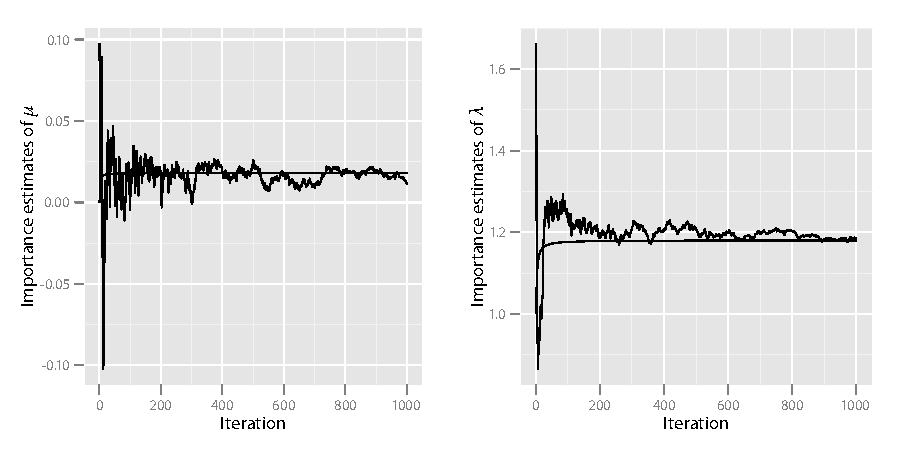
\includegraphics{fig/5-ndm}
  \caption{\smc estimates of means of distribution parameters for Normal
    model, Normal data}
  \label{fig:normal_dist_mean}
\end{figure}

\paragraph{Estimation of the normalizing constants} Let $Z_k$ denote the
normalizing constants of target distribution $\pi_k$ at iteration $k$. The
computation of likelihood function and prior $\pi_0$ was normalized,
therefore, the ratio $Z_{1000}/Z_0$ is exactly the normalizing constants of
the posterior distribution $\pi(\mu,\lambda)$ as in
equations~\eqref{eq:normal_posterior} and~\eqref{eq:laplace_posterior}. The
estimates of the normalizing constants using both \smc estimator in
equation~\eqref{eq:z_smc} and path sampling estimator in
equation~\eqref{eq:z_path} for the two models are plotted in
Figure~\ref{fig:normal_z}. Also shown in Figure~\ref{fig:normal_qq} is the
QQ-plot of the data against the theoretical quantile of the two model, with
parameters estimated form the \smc sampler. The first plot showed that both
\smc and path sampling estimates can perfectly distinguish between the two
models, as expected. However, the \smc estimates have considerably larger
variance than the path sampling estimates. The second plot showed that
Normal model indeed fit the data much better than the Laplace model.

\begin{figure}[htb]
  \centering
  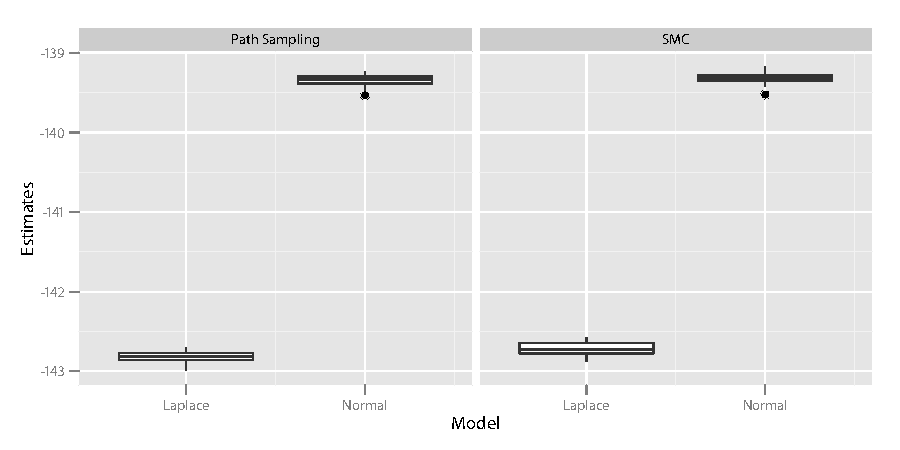
\includegraphics{fig/5-nz}
  \caption{Normalizing constants estimates of Normal data, using \smc and
    path sampling. The estimates from $100$ simulations are plotted.}
  \label{fig:normal_z}
\end{figure}

\begin{figure}[htb]
  \centering
  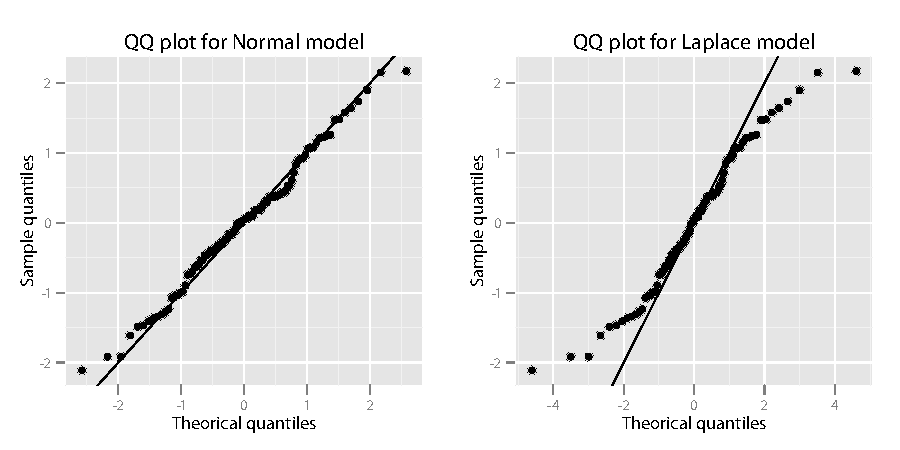
\includegraphics{fig/5-nqq}
  \caption{QQ-plots of data against the two model, Normal data}
  \label{fig:normal_qq}
\end{figure}

\subsubsection{Laplace data}

The data is simulated from the Laplace density, $\calL(0, \sqrt{2}/2)$. The
algorithm is as described in the last section. Analogy to
Figure~\ref{fig:normal_z} and~\ref{fig:normal_qq}, the estimates of
normalizing constants and QQ-plots for the data against the model are shown
in Figure~\ref{fig:laplace_z} and~\ref{fig:laplace_qq}. The results are
similar to the Normal data, except that this time the Laplace model is
preferable, as expected.

\begin{figure}[htb]
  \centering
  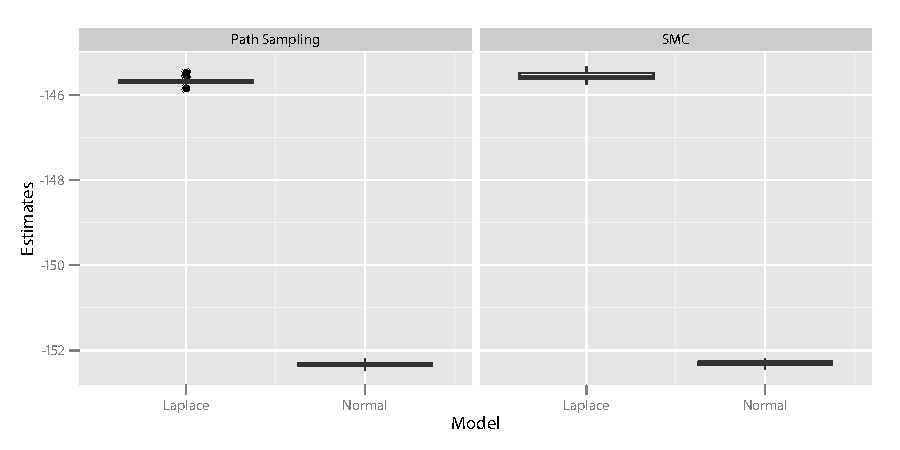
\includegraphics{fig/5-lz}
  \caption{Normalizing constants estimates of Laplace data, using \smc and
    path sampling. The estimates from $100$ simulations are plotted.}
  \label{fig:laplace_z}
\end{figure}

\begin{figure}[htb]
  \centering
  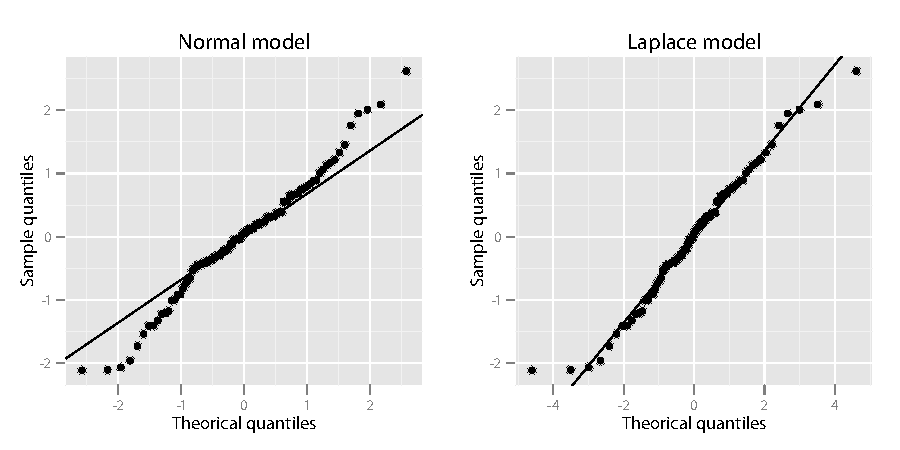
\includegraphics{fig/5-lqq}
  \caption{QQ-plots of data against the two model, Laplace data}
  \label{fig:laplace_qq}
\end{figure}

\subsection{Discussion}
\label{sub:Discussion}

As demonstrated in this chapter, it is possible to use \smc sampler and path
sampling estimator to do Bayesian model comparison. There are some aspects of
the estimator worth further investigation in the research follows here.

\paragraph{Quality of the estimator} In \textcite{DelMoral2006} and references
thereby, a central limited theorem was established for the importance sampling
estimator for $\Exp[\phi(x_n)]$, where $\phi(\cdot)$ is an arbitrary and $X_n$
is are from the distribution $\pi_n$ at step $n$ of \smc iterations. The
results was obtained under the assumption of certain resampling schemes.
However, to access the quality of path sampling estimator requires more than
that. It may be of interest at some stage to examine the Monte Carlo properly
of the estimator properly.

\paragraph{Efficiency} The \smc sampler requires considerable computation
resources. Though it is argued to be of order $O(N)$ where $N$ is the number
of particles, it often requires much more computation time than a \mcmc
algorithm with $N$ iterations. As always in practice, there is a trade-off
between quality of estimates and time consumed by the computation. Therefore
the methods proposed here will be less of interest if it only provide marginal
improvement in the quality of estimates compared to \mcmc, while it requires
far more computation resources. The efficiency or optimization of the proposed
methods will be of interest at some stage, though not immediately. It will be
of interest to investigate how to construct the ``path'' effectively. And
literatures in numerical integration is a possible source for inspiration.
Further, in the simple examples, the same \mha is used for each iteration when
doing the forward moves. However, it will probably be more efficient to
construct the forward kernel adaptively. And the well established literatures
in \mcmc are likely to be useful.

\paragraph{Estimating Bayes factor directly} In the simple example, the
normalizing constants are estimated for each posterior distribution
individually. It is possible to construct a path passing through the posterior
distributions of both models. And the ratio of normalizing constants can be
obtained directly. More interesting is the use these techniques in a
trans-dimensional setting. However the later part will not be the concern in
the near future.

\section{Summary}
\label{sec:5-Summary}

The first of further research will be establishing a general
framework for using the proposed methods to do Bayesian model comparison. This
includes solving a few problems,
\begin{enumerate}
  \item How to get the method work? This is a more technical problem. We need
    to get the methods work for less trivial problems and see how it works.
  \item Under what condition it will work? There is no method that can solve
    all problems. Every method is only valid under some assumptions or
    conditions.
  \item What is the property of the estimator in general? This will be a more
    difficult problem. Though theories on \smc and path sampling are both
    established in literature, the properties of the estimator obtained by
    combining them together are not known completely. At this stage it is
    difficult to tell when or how such theorems will be established.
\end{enumerate}
Further research following the problems raised above may contain optimization,
etc.
